% Created 2023-06-23 Fri 21:54
% Intended LaTeX compiler: pdflatex
\documentclass[11pt]{article}
\usepackage[utf8]{inputenc}
\usepackage[T1]{fontenc}
\usepackage{graphicx}
\usepackage{longtable}
\usepackage{wrapfig}
\usepackage{rotating}
\usepackage[normalem]{ulem}
\usepackage{amsmath}
\usepackage{amssymb}
\usepackage{capt-of}
\usepackage{hyperref}
\usepackage{todonotes}
\usepackage[brazil, american]{babel}
\usepackage{amsthm}
\author{Ieremies Vieira da Fonseca Romero}
\date{}
\title{Trabalho 4\\\medskip
\large Processamento Digital de Imagem}
\hypersetup{
 pdfauthor={Ieremies Vieira da Fonseca Romero},
 pdftitle={Trabalho 4},
 pdfkeywords={},
 pdfsubject={},
 pdfcreator={Emacs 28.2 (Org mode 9.6.1)}, 
 pdflang={English}}

% Setup for code blocks [1/2]

\usepackage{fvextra}

\fvset{%
  commandchars=\\\{\},
  highlightcolor=white!95!black!80!blue,
  breaklines=true,
  breaksymbol=\color{white!60!black}\tiny\ensuremath{\hookrightarrow}}

% Make line numbers smaller and grey.
\renewcommand\theFancyVerbLine{\footnotesize\color{black!40!white}\arabic{FancyVerbLine}}

\usepackage{xcolor}

% In case engrave-faces-latex-gen-preamble has not been run.
\providecolor{EfD}{HTML}{f7f7f7}
\providecolor{EFD}{HTML}{28292e}

% Define a Code environment to prettily wrap the fontified code.
\usepackage[breakable,xparse]{tcolorbox}
\DeclareTColorBox[]{Code}{o}%
{colback=EfD!98!EFD, colframe=EfD!95!EFD,
  fontupper=\footnotesize\setlength{\fboxsep}{0pt},
  colupper=EFD,
  IfNoValueTF={#1}%
  {boxsep=2pt, arc=2.5pt, outer arc=2.5pt,
    boxrule=0.5pt, left=2pt}%
  {boxsep=2.5pt, arc=0pt, outer arc=0pt,
    boxrule=0pt, leftrule=1.5pt, left=0.5pt},
  right=2pt, top=1pt, bottom=0.5pt,
  breakable}

% Support listings with captions
\usepackage{float}
\floatstyle{plain}
\newfloat{listing}{htbp}{lst}
\newcommand{\listingsname}{Listing}
\floatname{listing}{\listingsname}
\newcommand{\listoflistingsname}{List of Listings}
\providecommand{\listoflistings}{\listof{listing}{\listoflistingsname}}


% Setup for code blocks [2/2]: syntax highlighting colors

\newcommand\efstrut{\vrule height 2.1ex depth 0.8ex width 0pt}
\definecolor{EFD}{HTML}{000000}
\definecolor{EfD}{HTML}{ffffff}
\newcommand{\EFD}[1]{\textcolor{EFD}{#1}} % default
\definecolor{EFvp}{HTML}{000000}
\newcommand{\EFvp}[1]{\textcolor{EFvp}{#1}} % variable-pitch
\definecolor{EFh}{HTML}{7f7f7f}
\newcommand{\EFh}[1]{\textcolor{EFh}{#1}} % shadow
\definecolor{EFsc}{HTML}{228b22}
\newcommand{\EFsc}[1]{\textcolor{EFsc}{\textbf{#1}}} % success
\definecolor{EFw}{HTML}{ff8e00}
\newcommand{\EFw}[1]{\textcolor{EFw}{\textbf{#1}}} % warning
\definecolor{EFe}{HTML}{ff0000}
\newcommand{\EFe}[1]{\textcolor{EFe}{\textbf{#1}}} % error
\definecolor{EFl}{HTML}{ff0000}
\newcommand{\EFl}[1]{\textcolor{EFl}{#1}} % link
\definecolor{EFlv}{HTML}{ff0000}
\newcommand{\EFlv}[1]{\textcolor{EFlv}{#1}} % link-visited
\definecolor{EFhi}{HTML}{ff0000}
\newcommand{\EFhi}[1]{\textcolor{EFhi}{#1}} % highlight
\definecolor{EFc}{HTML}{b22222}
\newcommand{\EFc}[1]{\textcolor{EFc}{#1}} % font-lock-comment-face
\definecolor{EFcd}{HTML}{b22222}
\newcommand{\EFcd}[1]{\textcolor{EFcd}{#1}} % font-lock-comment-delimiter-face
\definecolor{EFs}{HTML}{8b2252}
\newcommand{\EFs}[1]{\textcolor{EFs}{#1}} % font-lock-string-face
\definecolor{EFd}{HTML}{8b2252}
\newcommand{\EFd}[1]{\textcolor{EFd}{#1}} % font-lock-doc-face
\definecolor{EFm}{HTML}{008b8b}
\newcommand{\EFm}[1]{\textcolor{EFm}{#1}} % font-lock-doc-markup-face
\definecolor{EFk}{HTML}{9370db}
\newcommand{\EFk}[1]{\textcolor{EFk}{#1}} % font-lock-keyword-face
\definecolor{EFb}{HTML}{483d8b}
\newcommand{\EFb}[1]{\textcolor{EFb}{#1}} % font-lock-builtin-face
\definecolor{EFf}{HTML}{0000ff}
\newcommand{\EFf}[1]{\textcolor{EFf}{#1}} % font-lock-function-name-face
\definecolor{EFv}{HTML}{a0522d}
\newcommand{\EFv}[1]{\textcolor{EFv}{#1}} % font-lock-variable-name-face
\definecolor{EFt}{HTML}{228b22}
\newcommand{\EFt}[1]{\textcolor{EFt}{#1}} % font-lock-type-face
\definecolor{EFo}{HTML}{008b8b}
\newcommand{\EFo}[1]{\textcolor{EFo}{#1}} % font-lock-constant-face
\definecolor{EFwr}{HTML}{ff0000}
\newcommand{\EFwr}[1]{\textcolor{EFwr}{\textbf{#1}}} % font-lock-warning-face
\newcommand{\EFnc}[1]{#1} % font-lock-negation-char-face
\definecolor{EFpp}{HTML}{483d8b}
\newcommand{\EFpp}[1]{\textcolor{EFpp}{#1}} % font-lock-preprocessor-face
\newcommand{\EFrc}[1]{\textbf{#1}} % font-lock-regexp-grouping-construct
\newcommand{\EFrb}[1]{\textbf{#1}} % font-lock-regexp-grouping-backslash
\newcommand{\EFob}[1]{#1} % org-block
\newcommand{\EFobb}[1]{#1} % org-block-begin-line
\newcommand{\EFobe}[1]{#1} % org-block-end-line
\definecolor{EFOa}{HTML}{0000ff}
\newcommand{\EFOa}[1]{\textcolor{EFOa}{#1}} % outline-1
\definecolor{EFOb}{HTML}{a0522d}
\newcommand{\EFOb}[1]{\textcolor{EFOb}{#1}} % outline-2
\definecolor{EFOc}{HTML}{a020f0}
\newcommand{\EFOc}[1]{\textcolor{EFOc}{#1}} % outline-3
\definecolor{EFOd}{HTML}{b22222}
\newcommand{\EFOd}[1]{\textcolor{EFOd}{#1}} % outline-4
\definecolor{EFOe}{HTML}{228b22}
\newcommand{\EFOe}[1]{\textcolor{EFOe}{#1}} % outline-5
\definecolor{EFOf}{HTML}{008b8b}
\newcommand{\EFOf}[1]{\textcolor{EFOf}{#1}} % outline-6
\definecolor{EFOg}{HTML}{483d8b}
\newcommand{\EFOg}[1]{\textcolor{EFOg}{#1}} % outline-7
\definecolor{EFOh}{HTML}{8b2252}
\newcommand{\EFOh}[1]{\textcolor{EFOh}{#1}} % outline-8
\definecolor{EFhn}{HTML}{008b8b}
\newcommand{\EFhn}[1]{\textcolor{EFhn}{#1}} % highlight-numbers-number
\definecolor{EFhq}{HTML}{9370db}
\newcommand{\EFhq}[1]{\textcolor{EFhq}{#1}} % highlight-quoted-quote
\definecolor{EFhs}{HTML}{008b8b}
\newcommand{\EFhs}[1]{\textcolor{EFhs}{#1}} % highlight-quoted-symbol
\definecolor{EFrda}{HTML}{707183}
\newcommand{\EFrda}[1]{\textcolor{EFrda}{#1}} % rainbow-delimiters-depth-1-face
\definecolor{EFrdb}{HTML}{7388d6}
\newcommand{\EFrdb}[1]{\textcolor{EFrdb}{#1}} % rainbow-delimiters-depth-2-face
\definecolor{EFrdc}{HTML}{909183}
\newcommand{\EFrdc}[1]{\textcolor{EFrdc}{#1}} % rainbow-delimiters-depth-3-face
\definecolor{EFrdd}{HTML}{709870}
\newcommand{\EFrdd}[1]{\textcolor{EFrdd}{#1}} % rainbow-delimiters-depth-4-face
\definecolor{EFrde}{HTML}{907373}
\newcommand{\EFrde}[1]{\textcolor{EFrde}{#1}} % rainbow-delimiters-depth-5-face
\definecolor{EFrdf}{HTML}{6276ba}
\newcommand{\EFrdf}[1]{\textcolor{EFrdf}{#1}} % rainbow-delimiters-depth-6-face
\definecolor{EFrdg}{HTML}{858580}
\newcommand{\EFrdg}[1]{\textcolor{EFrdg}{#1}} % rainbow-delimiters-depth-7-face
\definecolor{EFrdh}{HTML}{80a880}
\newcommand{\EFrdh}[1]{\textcolor{EFrdh}{#1}} % rainbow-delimiters-depth-8-face
\definecolor{EFrdi}{HTML}{887070}
\newcommand{\EFrdi}[1]{\textcolor{EFrdi}{#1}} % rainbow-delimiters-depth-9-face
\usepackage[date=year]{biblatex}

\begin{document}

\maketitle


\section*{Introdução}
\label{sec:org52659e6}
O processamento digital de imagens é uma área de estudo fundamental em Ciência da Computação, que visa o tratamento e manipulação de imagens digitais por meio de técnicas e algoritmos computacionais.
A análise e processamento de imagens digitais é uma tarefa complexa e multidisciplinar, que envolve conhecimentos em matemática, estatística, computação gráfica, processamento de sinais e outras áreas correlatas.

O objetivo deste trabalho é apresentar uma série de processamentos básicos em imagens digitais, abordando desde a leitura e escrita de imagens até operações de filtragem.
Para o desenvolvimento das operações, será empregada a vetorização de comandos, que permite processar as imagens de forma mais eficiente e rápida, através da aplicação de operações vetoriais em vez de operações matriciais.

\section*{O programa}
\label{sec:org5f94a0c}
Neste trabalho, utilizamos as bibliotecas \texttt{numpy} 1.24.1 e OpenCV 4.7.0.72 utilizado via \texttt{cv2}.
\begin{Code}
\begin{Verbatim}
\color{EFD}\textcolor[HTML]{9370db}{import} cv2
\textcolor[HTML]{9370db}{import} numpy \textcolor[HTML]{9370db}{as} np
\end{Verbatim}
\end{Code}

Cada uma das preposições do enúnciado é resolvido por uma função contida no arquivo \texttt{funcs.py}.
Todas as funções possuem como primeiro parâmetro a imagem ou janela sob a qual ela irá atuar.

Para leitura e escrita das imagens, utilizaremos as seguintes funções do \texttt{cv2}.
\begin{Code}
\begin{Verbatim}
\color{EFD}\textcolor[HTML]{b22222}{\# read the pgm image}
cv2.\textcolor[HTML]{37474F}{\textbf{\textit{imread}}}(\textcolor[HTML]{8b2252}{'in.pgm'})
cv2.\textcolor[HTML]{37474F}{\textbf{\textit{imwrite}}}(\textcolor[HTML]{8b2252}{'out.pgm'}, img)
\end{Verbatim}
\end{Code}

\section*{Perspectiva}
\label{sec:orgde20c81}
Para essa primeira parte, o código está presente no arquivo \texttt{perspec.py}.
O primeiro passo é definir os pontos de origem e destino da projeção perspectiva:
\begin{Code}
\begin{Verbatim}
\color{EFD}\textcolor[HTML]{a0522d}{source} \textcolor[HTML]{9370db}{=} np.\textcolor[HTML]{37474F}{\textbf{\textit{float32}}}([[\textcolor[HTML]{29B6F6}{37}, \textcolor[HTML]{29B6F6}{51}], [\textcolor[HTML]{29B6F6}{342}, \textcolor[HTML]{29B6F6}{42}], [\textcolor[HTML]{29B6F6}{485}, \textcolor[HTML]{29B6F6}{467}], [\textcolor[HTML]{29B6F6}{73}, \textcolor[HTML]{29B6F6}{380}]])
\textcolor[HTML]{a0522d}{dest} \textcolor[HTML]{9370db}{=} np.\textcolor[HTML]{37474F}{\textbf{\textit{float32}}}([[\textcolor[HTML]{29B6F6}{0}, \textcolor[HTML]{29B6F6}{0}], [\textcolor[HTML]{29B6F6}{511}, \textcolor[HTML]{29B6F6}{0}], [\textcolor[HTML]{29B6F6}{511}, \textcolor[HTML]{29B6F6}{511}], [\textcolor[HTML]{29B6F6}{0}, \textcolor[HTML]{29B6F6}{511}]])
\end{Verbatim}
\end{Code}

Depois, podemos calcular a matriz de transformação usando a função \texttt{cv2.getPerspectiveTransform} pasando os pontos desejados como parâmetro.
\begin{Code}
\begin{Verbatim}
\color{EFD}\textcolor[HTML]{a0522d}{M} \textcolor[HTML]{9370db}{=} cv2.\textcolor[HTML]{37474F}{\textbf{\textit{getPerspectiveTransform}}}(src, dest)
\end{Verbatim}
\end{Code}

Por fim, aplicamos a projeção perspectiva em na imagem desejada.
\begin{Code}
\begin{Verbatim}
\color{EFD}\textcolor[HTML]{a0522d}{image} \textcolor[HTML]{9370db}{=} cv2.\textcolor[HTML]{37474F}{\textbf{\textit{imread}}}(\textcolor[HTML]{8b2252}{"img/baboon\_perspectiva.png"})
\textcolor[HTML]{a0522d}{output\_image} \textcolor[HTML]{9370db}{=} cv2.\textcolor[HTML]{37474F}{\textbf{\textit{warpPerspective}}}(image, \textcolor[HTML]{008b8b}{M}, (\textcolor[HTML]{29B6F6}{512}, \textcolor[HTML]{29B6F6}{512}))
cv2.\textcolor[HTML]{37474F}{\textbf{\textit{imwrite}}}(\textcolor[HTML]{8b2252}{"./out.png"}, output\_image)
\end{Verbatim}
\end{Code}

\section*{Transformações geométricas}
\label{sec:orgfc36f56}
A primeira parte do programa é determinar os parâmetros que utilizamos.
Para isso, fazemos uso da bilbioteca \texttt{argparse} disponível no python, a fim de declarar quais as ``flags'' e argumentos possíveis.
Dessa forma, no arquivo \texttt{arg\_parser.py}, definimos um \texttt{parser} e utilizamos o método \texttt{add\_argument} para declara cada um dos argumentos do programa.
São eles:
\begin{description}
\item[{Ângulo}] \texttt{-a}, ângulo de rotação medido em graus no sentido anti-horário.
\item[{Escala}] \texttt{-e}, fator de escala.
\item[{Dimensão}] \texttt{-d}, largura e altura da imagem resultante desejada.
\item[{Método de interpolação}] \texttt{-m}, pode ser \texttt{proximo} (vizinho mais próximo), \texttt{bilinear}, \texttt{bicubica} ou \texttt{lagrange}.
\item[{Entrada}] \texttt{-i}, caminho para a imagem a ser processada
\item[{Saída}] \texttt{-o}, caminho para a imagem a ser gerada.
\end{description}

Todas essas informações estão disponíveis utilizando \texttt{python prog.py -{}-help}.

Nosso programa principal, no arquivo \texttt{prog.py} conciste em pegar os parâmetros na variável \texttt{args} e chamar a função \texttt{scale\_and\_rotate\_image} com eles.
Esta, por sua vez, é quem realiza as duas transformações.

Primeiro passo é determinar algumas informações sobre a imagem que estamos trabalhando.
A utilizadade delas ficará mais clara logo após.
\begin{Code}
\begin{Verbatim}
\color{EFD}\textcolor[HTML]{b22222}{\# converter o ângulo de rotação para radianos}
\textcolor[HTML]{a0522d}{angle} \textcolor[HTML]{9370db}{=} np.\textcolor[HTML]{37474F}{\textbf{\textit{deg2rad}}}(angle)

\textcolor[HTML]{b22222}{\# Criar uma imagem com a dimensão dim}
\textcolor[HTML]{a0522d}{res} \textcolor[HTML]{9370db}{=} np.\textcolor[HTML]{37474F}{\textbf{\textit{zeros}}}((dim[\textcolor[HTML]{29B6F6}{1}], dim[\textcolor[HTML]{29B6F6}{0}], \textcolor[HTML]{29B6F6}{3}), np.\textit{uint8})

\textcolor[HTML]{b22222}{\# O centro da imagem de saída}
\textcolor[HTML]{a0522d}{center} \textcolor[HTML]{9370db}{=} (dim[\textcolor[HTML]{29B6F6}{0}] \textcolor[HTML]{9370db}{//} \textcolor[HTML]{29B6F6}{2}, dim[\textcolor[HTML]{29B6F6}{1}] \textcolor[HTML]{9370db}{//} \textcolor[HTML]{29B6F6}{2})

\textcolor[HTML]{b22222}{\# O centro da imagem de entrada}
\textcolor[HTML]{a0522d}{center\_in} \textcolor[HTML]{9370db}{=} (image.\textit{shape}[\textcolor[HTML]{29B6F6}{1}] \textcolor[HTML]{9370db}{//} \textcolor[HTML]{29B6F6}{2}, image.\textit{shape}[\textcolor[HTML]{29B6F6}{0}] \textcolor[HTML]{9370db}{//} \textcolor[HTML]{29B6F6}{2})
\end{Verbatim}
\end{Code}

Para operar as transformações, faremos o processo inverso: ao invés de determinar onde um pixel da entrada irá estar na saída, determinaremos de onde o pixel da saída irá tirar o seu valor.
Isso faz com que o processo de interpolação usado para preencher os espaços vazios fique mais fácil.
Mas para isso, precisaremos aplicar o inverso das operações.

Dessa forma, para cada ponto \texttt{(y,x)} da saída, realizaremos o seguinte processo: transladamos de forma que o centro da imagem fique no \texttt{(0,0)} e multiplicamos pelo inverso do fator de escala.
\begin{Code}
\begin{Verbatim}
\color{EFD}\textcolor[HTML]{a0522d}{coord} \textcolor[HTML]{9370db}{=} (
    (y \textcolor[HTML]{9370db}{-} center[\textcolor[HTML]{29B6F6}{0}]) \textcolor[HTML]{9370db}{/} scale\_factor,
    (x \textcolor[HTML]{9370db}{-} center[\textcolor[HTML]{29B6F6}{1}]) \textcolor[HTML]{9370db}{/} scale\_factor,
)
\end{Verbatim}
\end{Code}

Depois, utilizamos a matriz inversa da rotação para obter as seguintes equações: \(x' = cos(a)x + sin(a)y\) e \(y' = - sin(a)x + cos(a)y\).
\begin{Code}
\begin{Verbatim}
\color{EFD}\textcolor[HTML]{a0522d}{coord} \textcolor[HTML]{9370db}{=} (
    coord[\textcolor[HTML]{29B6F6}{0}] \textcolor[HTML]{9370db}{*} np.\textcolor[HTML]{37474F}{\textbf{\textit{cos}}}(angle) \textcolor[HTML]{9370db}{+} coord[\textcolor[HTML]{29B6F6}{1}] \textcolor[HTML]{9370db}{*} np.\textcolor[HTML]{37474F}{\textbf{\textit{sin}}}(angle),
    coord[\textcolor[HTML]{29B6F6}{1}] \textcolor[HTML]{9370db}{*} np.\textcolor[HTML]{37474F}{\textbf{\textit{cos}}}(angle) \textcolor[HTML]{9370db}{-} coord[\textcolor[HTML]{29B6F6}{0}] \textcolor[HTML]{9370db}{*} np.\textcolor[HTML]{37474F}{\textbf{\textit{sin}}}(angle),
)
\end{Verbatim}
\end{Code}

Enfim, desfazemos a translação realizada no começo, agora com o centro da imagem de entrada.
\begin{Code}
\begin{Verbatim}
\color{EFD}\textcolor[HTML]{a0522d}{coord} \textcolor[HTML]{9370db}{=} (
    coord[\textcolor[HTML]{29B6F6}{0}] \textcolor[HTML]{9370db}{+} center\_in[\textcolor[HTML]{29B6F6}{0}],
    coord[\textcolor[HTML]{29B6F6}{1}] \textcolor[HTML]{9370db}{+} center\_in[\textcolor[HTML]{29B6F6}{1}],
)
\end{Verbatim}
\end{Code}

Por fim, as coordenadas obtidas podem não ser inteiras, efetivamente se encontrando ``entre pixels'' da entrada.
Para isso, utilizamos o método de interpolação desejado para obter o valor do pixel da saída.
\begin{Code}
\begin{Verbatim}
\color{EFD}res[\textcolor[HTML]{a0522d}{y}, \textcolor[HTML]{a0522d}{x}] \textcolor[HTML]{9370db}{=} \textcolor[HTML]{37474F}{\textbf{interp}}(image, \textcolor[HTML]{9370db}{*}coord)
\end{Verbatim}
\end{Code}

\begin{figure}[htbp]
\centering
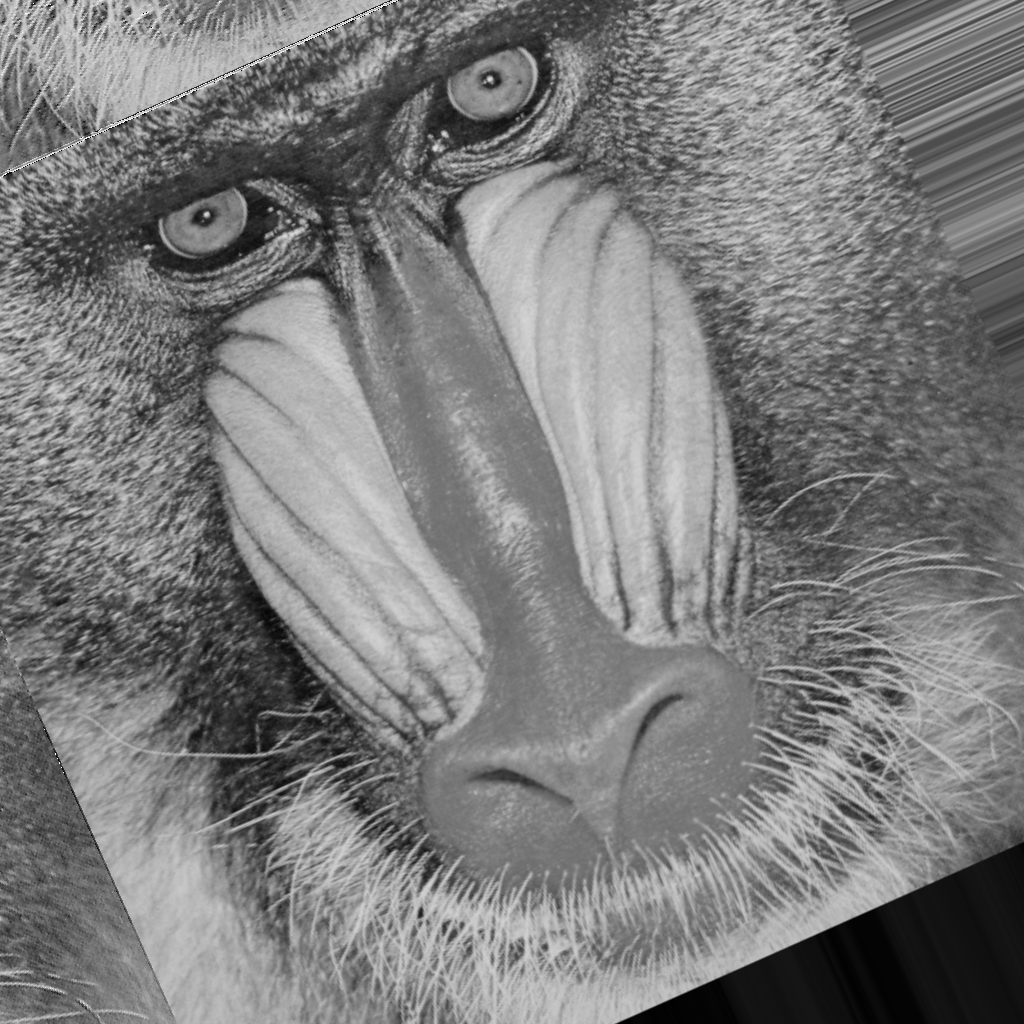
\includegraphics[width=.9\linewidth]{./out/baboon_rotated.png}
\caption{Resultado de uma escala por \(2.5\) e rotação de \(24\) graus.}
\end{figure}

\section*{Métodos de interpolação}
\label{sec:org500544c}
Cada método de interpolação é implementado por uma função que recebe a imagem original e as coordenadas \texttt{(x,y)} e retorna o valor do pixel para a saída.

O primeiro método de interpolação é utilizar o pixel mais próximo.
Em python, podemos fazer isso com o uso da função \texttt{round} que arredonda ao inteiro mais próximo.
\begin{Code}
\begin{Verbatim}
\color{EFD}\textcolor[HTML]{9370db}{def} \textcolor[HTML]{0000ff}{proximo}(\textcolor[HTML]{a0522d}{img}, \textcolor[HTML]{a0522d}{x}, \textcolor[HTML]{a0522d}{y}):
    \textcolor[HTML]{a0522d}{x} \textcolor[HTML]{9370db}{=} \textcolor[HTML]{483d8b}{\textbf{round}}(x)
    \textcolor[HTML]{a0522d}{y} \textcolor[HTML]{9370db}{=} \textcolor[HTML]{483d8b}{\textbf{round}}(y)
    \textcolor[HTML]{b22222}{\# caso o round passe dos limites da imagem original}
    \textcolor[HTML]{9370db}{if} x \textcolor[HTML]{9370db}{>=} img.\textit{shape}[\textcolor[HTML]{29B6F6}{0}] \textcolor[HTML]{9370db}{or} x \textcolor[HTML]{9370db}{<} \textcolor[HTML]{29B6F6}{0}:
        \textcolor[HTML]{9370db}{return} \textcolor[HTML]{29B6F6}{0}
    \textcolor[HTML]{9370db}{if} y \textcolor[HTML]{9370db}{>=} img.\textit{shape}[\textcolor[HTML]{29B6F6}{1}] \textcolor[HTML]{9370db}{or} x \textcolor[HTML]{9370db}{<} \textcolor[HTML]{29B6F6}{0}:
        \textcolor[HTML]{9370db}{return} \textcolor[HTML]{29B6F6}{0}
    \textcolor[HTML]{9370db}{return} img[x, y]
\end{Verbatim}
\end{Code}

\begin{figure}[htbp]
\centering
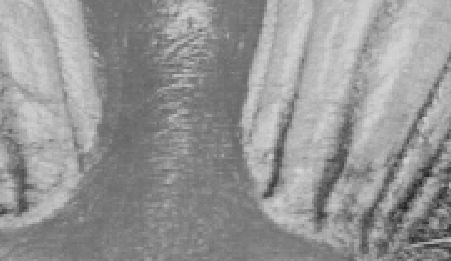
\includegraphics[width=.9\linewidth]{./out/proximo.png}
\caption{Zoom no resultado utilizando o método da interpolação do vizinho mais próximo. Observamos um efeito pixelado forte.}
\end{figure}

O segundo método é o \texttt{bilinear} que utiliza a média ponderada no inverso da distância dos quatro pontos mais próximos.
Este método tende a dar resultados mais ``suaves'' tendo em vista a natureza de média
\begin{Code}
\begin{Verbatim}
\color{EFD}\textcolor[HTML]{9370db}{def} \textcolor[HTML]{0000ff}{bilinear}(\textcolor[HTML]{a0522d}{img}, \textcolor[HTML]{a0522d}{x}, \textcolor[HTML]{a0522d}{y}):
    \textcolor[HTML]{a0522d}{dx} \textcolor[HTML]{9370db}{=} x \textcolor[HTML]{9370db}{-} \textcolor[HTML]{483d8b}{\textbf{int}}(x)
    \textcolor[HTML]{a0522d}{dy} \textcolor[HTML]{9370db}{=} y \textcolor[HTML]{9370db}{-} \textcolor[HTML]{483d8b}{\textbf{int}}(y)
    \textcolor[HTML]{a0522d}{x} \textcolor[HTML]{9370db}{=} \textcolor[HTML]{483d8b}{\textbf{int}}(x)  \textcolor[HTML]{b22222}{\# arredondar para baixo}
    \textcolor[HTML]{a0522d}{y} \textcolor[HTML]{9370db}{=} \textcolor[HTML]{483d8b}{\textbf{int}}(y)
    \textcolor[HTML]{a0522d}{res} \textcolor[HTML]{9370db}{=} (\textcolor[HTML]{29B6F6}{1} \textcolor[HTML]{9370db}{-} dx) \textcolor[HTML]{9370db}{*} (\textcolor[HTML]{29B6F6}{1} \textcolor[HTML]{9370db}{-} dy) \textcolor[HTML]{9370db}{*} img[x, y]
    \textcolor[HTML]{a0522d}{res} \textcolor[HTML]{9370db}{+=} dx \textcolor[HTML]{9370db}{*} (\textcolor[HTML]{29B6F6}{1} \textcolor[HTML]{9370db}{-} dy) \textcolor[HTML]{9370db}{*} img[x \textcolor[HTML]{9370db}{+} \textcolor[HTML]{29B6F6}{1}, y]
    \textcolor[HTML]{a0522d}{res} \textcolor[HTML]{9370db}{+=} (\textcolor[HTML]{29B6F6}{1} \textcolor[HTML]{9370db}{-} dx) \textcolor[HTML]{9370db}{*} dy \textcolor[HTML]{9370db}{*} img[x, y \textcolor[HTML]{9370db}{+} \textcolor[HTML]{29B6F6}{1}]
    \textcolor[HTML]{a0522d}{res} \textcolor[HTML]{9370db}{+=} dx \textcolor[HTML]{9370db}{*} dy \textcolor[HTML]{9370db}{*} img[x \textcolor[HTML]{9370db}{+} \textcolor[HTML]{29B6F6}{1}, y \textcolor[HTML]{9370db}{+} \textcolor[HTML]{29B6F6}{1}]
    \textcolor[HTML]{9370db}{return} res
\end{Verbatim}
\end{Code}

\begin{figure}[htbp]
\centering
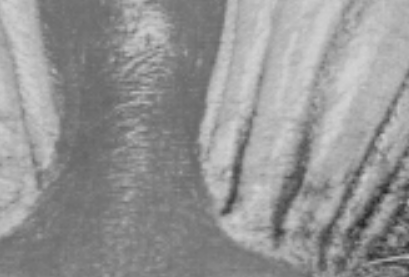
\includegraphics[width=.9\linewidth]{./out/bilinear.png}
\caption{Zoom no resultado utilizando o método da interpolação bilinear. Observamos que o resultado fica mais suave.}
\end{figure}

Não foi possível obter resultados satisfatórios com nossas implementações dos métodos bicúbicas nem do polinômio de lagrange.

\section*{Conclusão}
\label{sec:org309ee0b}
Neste trabalho, exploramos as transformações geométricas e a perspectiva como técnicas fundamentais no processamento digital de imagens. Utilizando as bibliotecas numpy e OpenCV, abordamos a aplicação de transformações como rotação, escala e projeção perspectiva em imagens digitais. Na seção de perspectiva, aprendemos como definir os pontos de origem e destino da projeção e aplicar a transformação utilizando a função cv2.getPerspectiveTransform. Isso nos permitiu realizar projeções perspectivas em imagens, obtendo resultados interessantes. Já nas transformações geométricas, exploramos a aplicação de interpolação para preencher os espaços vazios resultantes das transformações, utilizando métodos como o vizinho mais próximo e o bilinear. Essas técnicas são amplamente utilizadas em áreas como visão computacional, realidade virtual e processamento de imagens médicas, proporcionando uma compreensão essencial para a manipulação de imagens digitais e abrindo portas para futuras aplicações e estudos mais avançados.
\end{document}